\subsection{Ejercicio 8}
En la presente secci�n vamos a trabajar sobre un algoritmo de scheduling de tipo Round Robin pero que no permite la migraci�n de procesos entre
n�cleos. Para tal motivo se utiliza una cola de \texttt{READY} para cada core, donde una vez que el proceso llega se moviliza s�lo por esa cola.

Cuando el proceso es bloqueado debemos tener una manera de saber a qu� CPU pertenec�a dicho proceso, y para tal fin cada core tambi�n tiene una
cola de \texttt{BLOQUED}. Entonces, cuando un proceso es desbloqueado simplemente se lo busca en alguna de las listas \texttt{BLOQUED} de los cores,
y una vez que se lo encuentra se lo agrega a la cola \texttt{READY} correspondiente al core que ten�a esa tarea bloqueada. Esto hace que cada CPU
tenga un esquema de Round Robin de un s�lo core independiente del resto.

A continuaci�n mostramos un gr�fico correspondiente al procesamiento del lote de tareas \textit{lote5.tsk} para este nuevo scheduler.
Las tareas se encolan acorde a su momento de llegada y a la carga de los dem�s cores. Las tres primeras se cargan una en cada core, la cuarta
se carga en el primer core ya que todos estan igualmente cargados. Luego todas siguen ejecut�ndose en sus respectivos cores sin cambios de
lugar como es esperado.


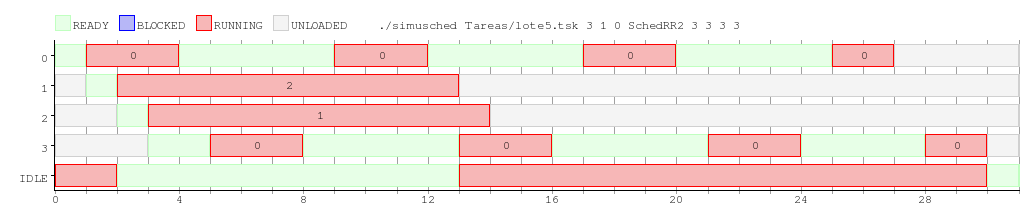
\includegraphics[width=1\textwidth]{./Graficos/ej8_1.png}
\begin{center}
 \textit{Cores = 3, Qantum = 3 cada core, CS = 1}.
\end{center}

Ahora, con el objetivo de comparar con la pol�tica de scheduling de una sola cola, vamos a correr el mismo lote para ver c�mo se comporta.
A continuaci�n se encuentra el gr�fico con la distribuci�n de las tareas.

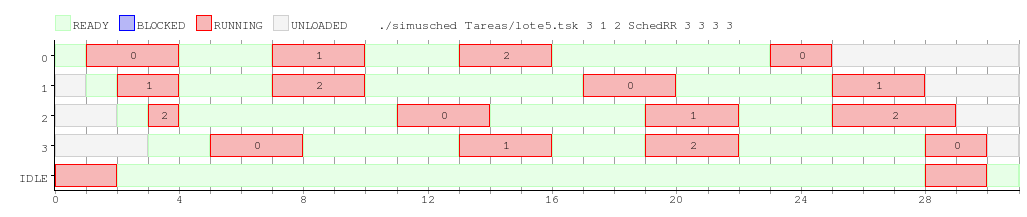
\includegraphics[width=1\textwidth]{./Graficos/ej8_2.png}
\begin{center}
 \textit{Cores = 3, Qantum = 3 cada core, CS = 1, CI = 2}.
\end{center}

Un detalle que vale la pena mencionar es que las tareas desde que iniciar hasta que finalizar estan asociadas a un solo core en el caso del
grafico uno. No ocurre asi en el gr�fico 2, en donde porciones de la tarea van cambiando de core, como se ve en el segundo gr�fico.

Para este lote de tareas en particular podemos apreciar que \texttt{SchedRR2} y \texttt{SchedRR} finalizan la ejecuci�n de todas las tareas
en un tiempo similar. Pero en el primer caso dos de las tareas finalizan r�pido, algo que no sucede en el segundo caso, sin contar que en
\texttt{SchedRR2} no hay costos por cambio de core, que s� presenta \texttt{SchedRR}.

Por otro lado, si bien es cierto que \texttt{SchedRR2} termina dos de las tres tareas m�s r�pido, tambi�n es cierto que esos cores quedan
inactivos el resto del tiempo (para este lote) algo que no es deseable. Esta comparativa nos brinda un indicio de que si bien \texttt{SchedRR2}
parece m�s eficiente, para algunos escenarios puede presentar desventajas con respecto a \texttt{SchedRR}, y dicho escenario es cuando
un core se queda con muchas tareas pendientes y los dem�s est�n ociosos.